\documentclass[a4paper,titlepage,11pt,twosides,floatssmall]{mwrep}
\usepackage[left=2.5cm,right=2.5cm,top=2.5cm,bottom=2.5cm]{geometry}
\usepackage[OT1]{fontenc}
\usepackage{polski}
\usepackage{amsmath}
\usepackage{amsfonts}
\usepackage{amssymb}
\usepackage{graphicx}
\usepackage{url}
\usepackage{tikz}
\usetikzlibrary{arrows,calc,decorations.markings,math,arrows.meta}
\usepackage{rotating}
\usepackage[percent]{overpic}
\usepackage[cp1250]{inputenc}
\usepackage{xcolor}
\usepackage{pgfplots}
\usetikzlibrary{pgfplots.groupplots}
\usepackage{listings}
\usepackage{matlab-prettifier}
\usepackage{siunitx}
\usepackage{placeins}
\definecolor{szary}{rgb}{0.95,0.95,0.95}
\sisetup{detect-weight,exponent-product=\cdot,output-decimal-marker={,},per-mode=symbol,binary-units=true,range-phrase={-},range-units=single}

%konfiguracje pakietu listings
\lstset{
	backgroundcolor=\color{szary},
	frame=single,
	breaklines=true,
}
\lstdefinestyle{customlatex}{
	basicstyle=\footnotesize\ttfamily,
	%basicstyle=\small\ttfamily,
}
\lstdefinestyle{customc}{
	breaklines=true,
	frame=tb,
	language=C,
	xleftmargin=0pt,
	showstringspaces=false,
	basicstyle=\small\ttfamily,
	keywordstyle=\bfseries\color{green!40!black},
	commentstyle=\itshape\color{purple!40!black},
	identifierstyle=\color{blue},
	stringstyle=\color{orange},
}
\lstdefinestyle{custommatlab}{
	captionpos=t,
	breaklines=true,
	frame=tb,
	xleftmargin=0pt,
	language=matlab,
	showstringspaces=false,
	%basicstyle=\footnotesize\ttfamily,
	basicstyle=\scriptsize\ttfamily,
	keywordstyle=\bfseries\color{green!40!black},
	commentstyle=\itshape\color{purple!40!black},
	identifierstyle=\color{blue},
	stringstyle=\color{orange},
}

%wymiar tekstu (bez �ywej paginy)
\textwidth 160mm \textheight 247mm

%ustawienia pakietu pgfplots
\pgfplotsset{
tick label style={font=\scriptsize},
label style={font=\small},
legend style={font=\small},
title style={font=\small}
}

\def\figurename{Rys.}
\def\tablename{Tab.}

%konfiguracja liczby p�ywaj�cych element�w
\setcounter{topnumber}{0}%2
\setcounter{bottomnumber}{3}%1
\setcounter{totalnumber}{5}%3
\renewcommand{\textfraction}{0.01}%0.2
\renewcommand{\topfraction}{0.95}%0.7
\renewcommand{\bottomfraction}{0.95}%0.3
\renewcommand{\floatpagefraction}{0.35}%0.5

\begin{document}
\frenchspacing
\pagestyle{uheadings}

%strona tytu�owa
\title{\bf Sprawozdanie z projektu i �wiczenia laboratoryjnego nr 2, zadanie nr 3\vskip 0.1cm}
\author{Mateusz Koro�, Ksawery Pasikowski, Mateusz Morusiewicz}
\date{2017}

\makeatletter
\renewcommand{\maketitle}{\begin{titlepage}
\begin{center}{\LARGE {\bf
Wydzia� Elektroniki i Technik Informacyjnych}}\\
\vspace{0.4cm}
{\LARGE {\bf Politechnika Warszawska}}\\
\vspace{0.3cm}
\end{center}
\vspace{5cm}
\begin{center}
{\bf \LARGE Projektowanie uk�ad�w sterowania\\ (projekt grupowy) \vskip 0.1cm}
\end{center}
\vspace{1cm}
\begin{center}
{\bf \LARGE \@title}
\end{center}
\vspace{2cm}
\begin{center}
{\bf \Large \@author \par}
\end{center}
\vspace*{\stretch{6}}
\begin{center}
\bf{\large{Warszawa, \@date\vskip 0.1cm}}
\end{center}
\end{titlepage}
}
\makeatother

\maketitle
\tableofcontents
\chapter{Zadanie 1.}
Poprawno�� warto�ci zosta�a potwierdzona poprzez sprawdzenie, czy obiekt, b�d�cy w punkcie pracy, pozostanie w nim, je�li zachowamy sta�e sterowanie, r�wne $ U_{pp} $, zosta�o to wykonane za pomoc� komendy:
\begin{lstlisting}[style=Matlab-editor]
y = symulacja_obiektu4Y(Upp, Upp, Ypp, Ypp)
\end{lstlisting}
Otrzymane $ y = 0,8 = Y_{pp} $, co potwierdza warto�ci $ U_{pp} $ oraz $ Y_{pp} $.
\documentclass[a4paper,11pt]{article}
\usepackage{pgfplots}
\usepackage{siunitx}
\sisetup{detect-weight,exponent-product=\cdot,output-decimal-marker={,},
	per-mode=symbol,binary-units=true,range-phrase={-},range-units=single}
\SendSettingsToPgf
\usetikzlibrary{pgfplots.groupplots}
\pgfplotsset{compat=1.11}
\usepgfplotslibrary{external}
\tikzexternalize

\textwidth 160mm \textheight 247mm

\pgfplotsset{width=\figurewidth,compat=1.11}
\pgfplotsset{
	tick label style={font=\tiny},
	label style={font=\footnotesize},
	legend style={font=\footnotesize},
	title style={font=\footnotesize}
}


\newcommand{\szer}{16cm}
\newcommand{\wys}{5.6cm}
\newcommand{\odstepionowy}{1.2cm}


\begin{document}

\tikzsetnextfilename{}

\begin{figure}[Odpowiedź na skok sterowania]
\tikzsetnextfilename{odpskokster}
\begin{tikzpicture}
\begin{groupplot}[group style={group size=1 by 2,vertical sep=\odstepionowy},
width=\szer,height=\wys]
%%1
\nextgroupplot
[xmin=1,xmax=300,ymin=-3,ymax=3,
xtick={0,50,...,300},
ytick={-3,-2.5,...,3},
ylabel={$y(k)$},
xlabel={$k$}]
\addplot[const plot,color=blue,semithick] file {datadir/zad2/odpowiedzi_skokowe/wyjscie_skok_0.8.txt};
\addplot[const plot,color=red,semithick] file {datadir/zad2/odpowiedzi_skokowe/wyjscie_skok_0.4.txt};
\addplot[const plot,color=green,semithick] file {datadir/zad2/odpowiedzi_skokowe/wyjscie_skok_-0.4.txt};
\addplot[const plot,color=purple,semithick] file {datadir/zad2/odpowiedzi_skokowe/wyjscie_skok_-0.8.txt};
\legend{$\Delta u = 0.8$,$\Delta u = 0.4$,$\Delta u = -0.4$, $\Delta u = -0.8$};

\nextgroupplot
[xmin=1,xmax=300,ymin=-1,ymax=1,
xtick={0,50,...,300},
ytick={-1,-0.5,...,1},
ylabel={$u(k)$},
xlabel={$k$}]
\addplot[const plot,color=blue,semithick] file {datadir/zad2/odpowiedzi_skokowe/sterowanie_skok_0.8.txt};
\addplot[const plot,color=red,semithick] file {datadir/zad2/odpowiedzi_skokowe/sterowanie_skok_0.4.txt};
\addplot[const plot,color=green,semithick] file {datadir/zad2/odpowiedzi_skokowe/sterowanie_skok_-0.4.txt};
\addplot[const plot,color=purple,semithick] file {datadir/zad2/odpowiedzi_skokowe/sterowanie_skok_-0.8.txt};
\legend{$\Delta u = 0.8$,$\Delta u = 0.4$,$\Delta u = -0.4$, $\Delta u = -0.8$};
\end{groupplot}
\end{tikzpicture}
\end{figure}


\begin{figure}[Charakterystyka statyczna]
\tikzsetnextfilename{charstat}
\begin{tikzpicture}
\begin{groupplot}[group style={group size=1 by 2,vertical sep=\odstepionowy},
width=\szer,height=\wys]
%%1
\nextgroupplot
[xmin=-1,xmax=1,ymin=-4,ymax=0.5,
xtick={-1,-0.5,...,1},
ytick={-4,-3.5,...,3},
ylabel={$y(u)$},
xlabel={$u$}]
\addplot[const plot,color=blue,semithick] file {datadir/zad2/char_stat/char_stat.txt};
\legend{ $y(u)$ }
\end{groupplot}
\end{tikzpicture}
\end{figure}

\end{document}

\documentclass[a4paper,11pt]{article}
\usepackage{pgfplots}
\usepackage{siunitx}
\sisetup{detect-weight,exponent-product=\cdot,output-decimal-marker={,},
	per-mode=symbol,binary-units=true,range-phrase={-},range-units=single}
\SendSettingsToPgf
\usetikzlibrary{pgfplots.groupplots}
\pgfplotsset{compat=1.11}
\usepgfplotslibrary{external}
\tikzexternalize

\textwidth 160mm \textheight 247mm

\pgfplotsset{width=\figurewidth,compat=1.11}
\pgfplotsset{
	tick label style={font=\tiny},
	label style={font=\footnotesize},
	legend style={font=\footnotesize},
	title style={font=\footnotesize}
}


\newcommand{\szer}{16cm}
\newcommand{\wys}{5.6cm}
\newcommand{\odstepionowy}{1.2cm}


\begin{document}

\tikzsetnextfilename{}

\begin{figure}[Odpowiedź toru u1 - y1]
\tikzsetnextfilename{zad3_u1y1}
\begin{tikzpicture}
\begin{groupplot}[group style={group size=1 by 2,vertical sep=\odstepionowy},
width=\szer,height=\wys]
%%1
\nextgroupplot
[xmin=1,xmax=400,ymin=0,ymax=0.3,
xtick={0,50,...,800},
ytick={0,0.05,...,0.3},
ylabel={$s^{1,1}(k)$},
xlabel={$k$}]
\addplot[const plot,color=blue,semithick] file {datadir/S_T1_G1.txt};
\addplot[const plot,color=red,densely dashed] file {datadir/Sapr_T1_G1.txt};
\legend{$s$,$s_{apr}$}
\end{groupplot}
\end{tikzpicture}
\end{figure}

\begin{figure}[Odpowiedź skokowa toru u1 - y2]
\tikzsetnextfilename{zad3_u1y2}
\begin{tikzpicture}
\begin{groupplot}[group style={group size=1 by 2,vertical sep=\odstepionowy},
width=\szer,height=\wys]
%%1
\nextgroupplot
[xmin=1,xmax=400,ymin=0,ymax=0.3,
xtick={0,50,...,800},
ytick={0,0.05,...,0.3},
ylabel={$s^{1,2}(k)$},
xlabel={$k$}]
\addplot[const plot,color=blue,semithick] file {datadir/S_T2_G1.txt};
\addplot[const plot,color=red,densely dashed] file {datadir/Sapr_T2_G1.txt};
\legend{$s$,$s_{apr}$}
\end{groupplot}
\end{tikzpicture}
\end{figure}


\begin{figure}[Odpowiedź skokowa toru u2 - y1]
\tikzsetnextfilename{zad3_u2y1}
\begin{tikzpicture}
\begin{groupplot}[group style={group size=1 by 2,vertical sep=\odstepionowy},
width=\szer,height=\wys]
%%1
\nextgroupplot
[xmin=1,xmax=400,ymin=0,ymax=0.3,
xtick={0,50,...,800},
ytick={0,0.05,...,0.3},
ylabel={$s^{2,1}(k)$},
xlabel={$k$}]
\addplot[const plot,color=blue,semithick] file {datadir/S_T1_G2.txt};
\addplot[const plot,color=red,densely dashed] file {datadir/Sapr_T1_G2.txt};
\legend{$s$,$s_{apr}$}
\end{groupplot}
\end{tikzpicture}
\end{figure}

\begin{figure}[Odpowiedź skokowa toru u2 - y2]
\tikzsetnextfilename{zad3_u2y2}
\begin{tikzpicture}
\begin{groupplot}[group style={group size=1 by 2,vertical sep=\odstepionowy},
width=\szer,height=\wys]
%%1
\nextgroupplot
[xmin=1,xmax=400,ymin=0,ymax=0.3,
xtick={0,50,...,800},
ytick={0,0.05,...,0.3},
ylabel={$s^{2,2}(k)$},
xlabel={$k$}]
\addplot[const plot,color=blue,semithick] file {datadir/S_T2_G2.txt};
\addplot[const plot,color=red,densely dashed] file {datadir/Sapr_T2_G2.txt};
\legend{$s$,$s_{apr}$}
\end{groupplot}
\end{tikzpicture}
\end{figure}


\begin{figure}[Błędy aproksymacji]
\tikzsetnextfilename{zad3_aproks}
\begin{tikzpicture}
\begin{groupplot}[group style={group size=1 by 4,vertical sep=\odstepionowy},
width=\szer,height=\wys]
%%1
\nextgroupplot
[xmin=1,xmax=30,ymin=0,ymax=1.5,
xtick={0,5,...,40},
ymode=log,
log ticks with fixed point,
ylabel={$E_{1,1}(Td)$},
xlabel={$Td$}]
\addplot[const plot,color=blue,semithick] file {datadir/E_T1_G1_69.txt};
%%1
\nextgroupplot
[xmin=1,xmax=30,ymin=0,ymax=1.5,
xtick={0,5,...,40},
ymode=log,
log ticks with fixed point,
ylabel={$E_{1,2}(Td)$},
xlabel={$Td$}]
\addplot[const plot,color=blue,semithick] file {datadir/E_T2_G1_69.txt};
%%1
\nextgroupplot
[xmin=1,xmax=40,ymin=0,ymax=1.5,
xtick={0,5,...,40},
ymode=log,
log ticks with fixed point,
ylabel={$E_{2,1}(Td)$},
xlabel={$Td$}]
\addplot[const plot,color=blue,semithick] file {datadir/E_T1_G2_74.txt};
%%1
\nextgroupplot
[xmin=1,xmax=40,ymin=0,ymax=1.5,
xtick={0,5,...,40},
ymode=log,
log ticks with fixed point,
ylabel={$E_{2,2}(Td)$},
xlabel={$Td$}]
\addplot[const plot,color=blue,semithick] file {datadir/E_T2_G2_74.txt};

\end{groupplot}
\end{tikzpicture}
\end{figure}

\end{document}

\documentclass[a4paper,11pt]{article}
\usepackage{pgfplots}
\usepackage{siunitx}
\sisetup{detect-weight,exponent-product=\cdot,output-decimal-marker={,},
	per-mode=symbol,binary-units=true,range-phrase={-},range-units=single}
\SendSettingsToPgf
\usetikzlibrary{pgfplots.groupplots}
\pgfplotsset{compat=1.11}
\usepgfplotslibrary{external}
\tikzexternalize

\textwidth 160mm \textheight 247mm

\pgfplotsset{width=\figurewidth,compat=1.11}
\pgfplotsset{
	tick label style={font=\tiny},
	label style={font=\footnotesize},
	legend style={font=\footnotesize},
	title style={font=\footnotesize}
}


\newcommand{\szer}{16cm}
\newcommand{\wys}{5.6cm}
\newcommand{\odstepionowy}{1.2cm}
\newcommand{\odstepoziomy}{1.2cm}





\begin{document}

\tikzsetnextfilename{}

\begin{figure}[Regulator DMC bez zakłócenia]
\tikzsetnextfilename{zad4_dmc}
\begin{tikzpicture}
\begin{groupplot}[group style={group size=1 by 2,vertical sep=\odstepionowy, horizontal sep=\odstepoziomy},
width=\szer,height=\wys]
%%1
\nextgroupplot
[xmin=1,xmax=600,ymin=30,ymax=44,
xtick={0, 50, 100, 150, 200, 250, 300, 350, 400, 450, 500, 550, 600},
ytick={30,32,34, 36,38,40,42,44},
ylabel={$y(t), y_{zad}(t)$},
xlabel={$t$}]
\addplot[const plot,color=red,semithick] file {datadir/zad4_y.txt};
\addplot[const plot,color=blue,densely dashed] file {datadir/zad4_yzad.txt};
\legend{$y(t)$,$y_{zad}(t)$}
\nextgroupplot
%%2
[xmin=1,xmax=600,ymin=0,ymax=100,
xtick={0, 50, 100, 150, 200, 250, 300, 350, 400, 450, 500, 550, 600},
ytick={0,10,20,30,40,50,60,70,80,90,100},
ylabel={$u(t)$},
xlabel={$t$}]
\addplot[const plot,color=red,semithick] file {datadir/zad4_u.txt};

\end{groupplot}
\end{tikzpicture}
\end{figure}

\end{document}

\documentclass[a4paper,11pt]{article}
\usepackage{pgfplots}
\usepackage{siunitx}
\sisetup{detect-weight,exponent-product=\cdot,output-decimal-marker={,},
	per-mode=symbol,binary-units=true,range-phrase={-},range-units=single}
\SendSettingsToPgf
\usetikzlibrary{pgfplots.groupplots}
\pgfplotsset{compat=1.11}
\usepgfplotslibrary{external}
\tikzexternalize

\textwidth 160mm \textheight 247mm

\pgfplotsset{width=\figurewidth,compat=1.11}
\pgfplotsset{
	tick label style={font=\tiny},
	label style={font=\footnotesize},
	legend style={font=\footnotesize},
	title style={font=\footnotesize}
}


\newcommand{\szer}{16cm}
\newcommand{\wys}{3.6cm}
\newcommand{\odstepionowy}{1.2cm}


\begin{document}

\tikzsetnextfilename{}


\begin{figure}[PID]
\tikzsetnextfilename{zad5_pid}
\begin{tikzpicture}
\begin{groupplot}[group style={group size=1 by 8,vertical sep=\odstepionowy},
width=\szer,height=\wys]
%%1
\nextgroupplot
[xmin=1,xmax=800,ymin=-1,ymax=2,
xtick={0,100,...,800},
ytick={-10,-9,...,10},
ylabel={$y_{1}(t)$},
xlabel={$t$}]

\addplot[const plot,color=red,semithick] file {../wykresy_pliki/zad5/PID/zad5PID_y1.txt};
\addplot[const plot,color=blue,densely dashed] file {../wykresy_pliki/zad5/PID/zad5PID_yzad1.txt};
\legend{$y_{1}(t)$,$y_{1 zad}(t)$}

\nextgroupplot
[xmin=1,xmax=800,ymin=-1,ymax=2,
xtick={0,100,...,800},
ytick={-10,-9,...,10},
ylabel={$y_{2}(t)$},
xlabel={$t$}]

\addplot[const plot,color=red,semithick] file {../wykresy_pliki/zad5/PID/zad5PID_y2.txt};
\addplot[const plot,color=blue,densely dashed] file {../wykresy_pliki/zad5/PID/zad5PID_yzad2.txt};
\legend{$y_2(t)$,$y_{2 zad}(t)$}


\nextgroupplot
[xmin=1,xmax=800,ymin=-1,ymax=2,
xtick={0,100,...,800},
ytick={-10,-9,...,10},
ylabel={$y_3(t)$},
xlabel={$t$}]

\addplot[const plot,color=red,semithick] file {../wykresy_pliki/zad5/PID/zad5PID_y3.txt};
\addplot[const plot,color=blue,densely dashed] file {../wykresy_pliki/zad5/PID/zad5PID_yzad3.txt};
\legend{$y_3(t)$,$y_{3 zad}(t)$}


%%1
\nextgroupplot
[xmin=1,xmax=800,ymin=-5,ymax=5,
xtick={0,100,...,800},
ytick={-10,-7.5,...,10},
ylabel={$u_1(t)$},
xlabel={$t$}]

\addplot[const plot,color=red,semithick] file {../wykresy_pliki/zad5/PID/zad5PID_u1.txt};
\legend{$u_1(t)$}


\nextgroupplot
[xmin=1,xmax=800,ymin=-5,ymax=5,
xtick={0,100,...,800},
ytick={-10,-7.5,...,10},
ylabel={$u_2(t)$},
xlabel={$t$}]

\addplot[const plot,color=red,semithick] file {../wykresy_pliki/zad5/PID/zad5PID_u2.txt};
\legend{$u_2(t)$}


\nextgroupplot
[xmin=1,xmax=800,ymin=-5,ymax=5,
xtick={0,100,...,800},
ytick={-10,-7.5,...,10},
ylabel={$u_4(t)$},
xlabel={$t$}]

\addplot[const plot,color=red,semithick] file {../wykresy_pliki/zad5/PID/zad5PID_u4.txt};
\legend{$u_4(t)$}



\end{groupplot}
\end{tikzpicture}
\end{figure}



\begin{figure}[DMC]
\tikzsetnextfilename{zad5_dmc}
\begin{tikzpicture}
\begin{groupplot}[group style={group size=1 by 8,vertical sep=\odstepionowy},
width=\szer,height=\wys]
%%1
\nextgroupplot
[xmin=1,xmax=800,ymin=-1,ymax=2,
xtick={0,100,...,800},
ytick={-10,-9,...,10},
ylabel={$y_{1}(t)$},
xlabel={$t$}]

\addplot[const plot,color=red,semithick] file {../wykresy_pliki/zad5/DMC/zad5DMC_y1.txt};
\addplot[const plot,color=blue,densely dashed] file {../wykresy_pliki/zad5/DMC/zad5DMC_yzad1.txt};
\legend{$y_{1}(t)$,$y_{1 zad}(t)$}

\nextgroupplot
[xmin=1,xmax=800,ymin=-1,ymax=2,
xtick={0,100,...,800},
ytick={-10,-9,...,10},
ylabel={$y_{2}(t)$},
xlabel={$t$}]

\addplot[const plot,color=red,semithick] file {../wykresy_pliki/zad5/DMC/zad5DMC_y2.txt};
\addplot[const plot,color=blue,densely dashed] file {../wykresy_pliki/zad5/DMC/zad5DMC_yzad2.txt};
\legend{$y_2(t)$,$y_{2 zad}(t)$}


\nextgroupplot
[xmin=1,xmax=800,ymin=-1,ymax=2,
xtick={0,100,...,800},
ytick={-10,-9,...,10},
ylabel={$y_3(t)$},
xlabel={$t$}]

\addplot[const plot,color=red,semithick] file {../wykresy_pliki/zad5/DMC/zad5DMC_y3.txt};
\addplot[const plot,color=blue,densely dashed] file {../wykresy_pliki/zad5/DMC/zad5DMC_yzad3.txt};
\legend{$y_3(t)$,$y_{3 zad}(t)$}


%%1
\nextgroupplot
[xmin=1,xmax=800,ymin=-5,ymax=5,
xtick={0,100,...,800},
ytick={-10,-7.5,...,10},
ylabel={$u_1(t)$},
xlabel={$t$}]

\addplot[const plot,color=red,semithick] file {../wykresy_pliki/zad5/DMC/zad5DMC_u1.txt};
\legend{$u_1(t)$}


\nextgroupplot
[xmin=1,xmax=800,ymin=-5,ymax=5,
xtick={0,100,...,800},
ytick={-10,-7.5,...,10},
ylabel={$u_2(t)$},
xlabel={$t$}]

\addplot[const plot,color=red,semithick] file {../wykresy_pliki/zad5/DMC/zad5DMC_u2.txt};
\legend{$u_2(t)$}

\nextgroupplot
[xmin=1,xmax=800,ymin=-5,ymax=5,
xtick={0,100,...,800},
ytick={-10,-7.5,...,10},
ylabel={$u_3(t)$},
xlabel={$t$}]

\addplot[const plot,color=red,semithick] file {../wykresy_pliki/zad5/DMC/zad5DMC_u3.txt};
\legend{$u_3(t)$}


\nextgroupplot
[xmin=1,xmax=800,ymin=-5,ymax=5,
xtick={0,100,...,800},
ytick={-10,-7.5,...,10},
ylabel={$u_4(t)$},
xlabel={$t$}]

\addplot[const plot,color=red,semithick] file {../wykresy_pliki/zad5/DMC/zad5DMC_u4.txt};
\legend{$u_4(t)$}



\end{groupplot}
\end{tikzpicture}
\end{figure}



\end{document}

\documentclass[a4paper,11pt]{article}
\usepackage{pgfplots}
\usepackage{siunitx}
\sisetup{detect-weight,exponent-product=\cdot,output-decimal-marker={,},
	per-mode=symbol,binary-units=true,range-phrase={-},range-units=single}
\SendSettingsToPgf
\usetikzlibrary{pgfplots.groupplots}
\pgfplotsset{compat=1.11}
\usepgfplotslibrary{external}
\tikzexternalize

\textwidth 160mm \textheight 247mm

\pgfplotsset{width=\figurewidth,compat=1.11}
\pgfplotsset{
	tick label style={font=\tiny},
	label style={font=\footnotesize},
	legend style={font=\footnotesize},
	title style={font=\footnotesize}
}


\newcommand{\szer}{16cm}
\newcommand{\wys}{5.6cm}
\newcommand{\odstepionowy}{1.2cm}


\begin{document}

\tikzsetnextfilename{}

\begin{figure}[DMC]
\tikzsetnextfilename{zad6DMC_lr_2}
\begin{tikzpicture}
\begin{groupplot}[group style={group size=1 by 2,vertical sep=\odstepionowy},
width=\szer,height=\wys]
%%1
\nextgroupplot
[xmin=1,xmax=800,ymin=-5,ymax=3,
xtick={0,50,...,800},
ytick={-5,-4,...,3},
ylabel={$y(k)$},
xlabel={$k$}]
\addplot[const plot,color=red,semithick] file {datadir/zad6/wyjscie_lr_2.txt};
\addplot[const plot,color=blue,semithick] file {datadir/zad6/wartosc_zadana.txt};
\legend{$y(k)$,$y_{zad}(k)$};

\nextgroupplot
[xmin=1,xmax=800,ymin=-2,ymax=2,
xtick={0,50,...,800},
ytick={-2,-1,...,2},
ylabel={$u(k)$},
xlabel={$k$}]
\addplot[const plot,color=red,semithick] file {datadir/zad6/sterowanie_lr_2.txt};
\legend{$u(k)$};
\end{groupplot}
\end{tikzpicture}
\end{figure}

\begin{figure}[DMC]
\tikzsetnextfilename{zad6DMC_lr_3}
\begin{tikzpicture}
\begin{groupplot}[group style={group size=1 by 2,vertical sep=\odstepionowy},
width=\szer,height=\wys]
%%1
\nextgroupplot
[xmin=1,xmax=800,ymin=-5,ymax=3,
xtick={0,50,...,800},
ytick={-5,-4,...,3},
ylabel={$y(k)$},
xlabel={$k$}]
\addplot[const plot,color=red,semithick] file {datadir/zad6/wyjscie_lr_3.txt};
\addplot[const plot,color=blue,semithick] file {datadir/zad6/wartosc_zadana.txt};
\legend{$y(k)$,$y_{zad}(k)$};

\nextgroupplot
[xmin=1,xmax=800,ymin=-2,ymax=2,
xtick={0,50,...,800},
ytick={-2,-1,...,2},
ylabel={$u(k)$},
xlabel={$k$}]
\addplot[const plot,color=red,semithick] file {datadir/zad6/sterowanie_lr_3.txt};
\legend{$u(k)$};
\end{groupplot}
\end{tikzpicture}
\end{figure}

\begin{figure}[DMC]
\tikzsetnextfilename{zad6DMC_lr_4}
\begin{tikzpicture}
\begin{groupplot}[group style={group size=1 by 2,vertical sep=\odstepionowy},
width=\szer,height=\wys]
%%1
\nextgroupplot
[xmin=1,xmax=800,ymin=-5,ymax=3,
xtick={0,50,...,800},
ytick={-5,-4,...,3},
ylabel={$y(k)$},
xlabel={$k$}]
\addplot[const plot,color=red,semithick] file {datadir/zad6/wyjscie_lr_4.txt};
\addplot[const plot,color=blue,semithick] file {datadir/zad6/wartosc_zadana.txt};
\legend{$y(k)$,$y_{zad}(k)$};

\nextgroupplot
[xmin=1,xmax=800,ymin=-2,ymax=2,
xtick={0,50,...,800},
ytick={-2,-1,...,2},
ylabel={$u(k)$},
xlabel={$k$}]
\addplot[const plot,color=red,semithick] file {datadir/zad6/sterowanie_lr_4.txt};
\legend{$u(k)$};
\end{groupplot}
\end{tikzpicture}
\end{figure}


\begin{figure}[DMC]
\tikzsetnextfilename{zad6DMC_lr_5}
\begin{tikzpicture}
\begin{groupplot}[group style={group size=1 by 2,vertical sep=\odstepionowy},
width=\szer,height=\wys]
%%1
\nextgroupplot
[xmin=1,xmax=800,ymin=-5,ymax=3,
xtick={0,50,...,800},
ytick={-5,-4,...,3},
ylabel={$y(k)$},
xlabel={$k$}]
\addplot[const plot,color=red,semithick] file {datadir/zad6/wyjscie_lr_5.txt};
\addplot[const plot,color=blue,semithick] file {datadir/zad6/wartosc_zadana.txt};
\legend{$y(k)$,$y_{zad}(k)$};

\nextgroupplot
[xmin=1,xmax=800,ymin=-2,ymax=2,
xtick={0,50,...,800},
ytick={-2,-1,...,2},
ylabel={$u(k)$},
xlabel={$k$}]
\addplot[const plot,color=red,semithick] file {datadir/zad6/sterowanie_lr_5.txt};
\legend{$u(k)$};
\end{groupplot}
\end{tikzpicture}
\end{figure}

\begin{figure}[DMC]
\tikzsetnextfilename{zad6DMC_odp1}
\begin{tikzpicture}
\begin{groupplot}[group style={group size=1 by 2,vertical sep=\odstepionowy},
width=\szer,height=\wys]

\nextgroupplot
[xmin=1,xmax=800,ymin=-2,ymax=6,
xtick={0,50,...,800},
ytick={-2,-1,...,6},
ylabel={$y(k)$},
xlabel={$k$}]
\addplot[const plot,color=red,semithick] file {datadir/zad6/odpowiedzi/wyjscie_skok_-1_-0.75.txt};
\legend{$y(k)$};
\end{groupplot}
\end{tikzpicture}
\end{figure}


\begin{figure}[DMC]
\tikzsetnextfilename{zad6DMC_odp2}
\begin{tikzpicture}
\begin{groupplot}[group style={group size=1 by 2,vertical sep=\odstepionowy},
width=\szer,height=\wys]

\nextgroupplot
[xmin=1,xmax=800,ymin=-2,ymax=6,
xtick={0,50,...,800},
ytick={-2,-1,...,6},
ylabel={$y(k)$},
xlabel={$k$}]
\addplot[const plot,color=red,semithick] file {datadir/zad6/odpowiedzi/wyjscie_skok_0.75_1.txt};
\legend{$y(k)$};
\end{groupplot}
\end{tikzpicture}
\end{figure}

\begin{figure}[DMC]
\tikzsetnextfilename{zad6DMC_odp3}
\begin{tikzpicture}
\begin{groupplot}[group style={group size=1 by 2,vertical sep=\odstepionowy},
width=\szer,height=\wys]

\nextgroupplot
[xmin=1,xmax=800,ymin=-2,ymax=6,
xtick={0,50,...,800},
ytick={-2,-1,...,6},
ylabel={$y(k)$},
xlabel={$k$}]
\addplot[const plot,color=red,semithick] file {datadir/zad6/odpowiedzi/wyjscie_skok_-0.6_-0.23.txt};
\legend{$y(k)$};
\end{groupplot}
\end{tikzpicture}
\end{figure}


\begin{figure}[DMC]
\tikzsetnextfilename{zad6DMC_odp4}
\begin{tikzpicture}
\begin{groupplot}[group style={group size=1 by 2,vertical sep=\odstepionowy},
width=\szer,height=\wys]

\nextgroupplot
[xmin=1,xmax=800,ymin=-2,ymax=6,
xtick={0,50,...,800},
ytick={-2,-1,...,6},
ylabel={$y(k)$},
xlabel={$k$}]
\addplot[const plot,color=red,semithick] file {datadir/zad6/odpowiedzi/wyjscie_skok_-0.6_-0.4.txt};
\legend{$y(k)$};
\end{groupplot}
\end{tikzpicture}
\end{figure}


\begin{figure}[DMC]
\tikzsetnextfilename{zad6DMC_odp5}
\begin{tikzpicture}
\begin{groupplot}[group style={group size=1 by 2,vertical sep=\odstepionowy},
width=\szer,height=\wys]

\nextgroupplot
[xmin=1,xmax=800,ymin=-2,ymax=6,
xtick={0,50,...,800},
ytick={-2,-1,...,6},
ylabel={$y(k)$},
xlabel={$k$}]
\addplot[const plot,color=red,semithick] file {datadir/zad6/odpowiedzi/wyjscie_skok_-0.4_-0.23.txt};
\legend{$y(k)$};
\end{groupplot}
\end{tikzpicture}
\end{figure}


\begin{figure}[DMC]
\tikzsetnextfilename{zad6DMC_odp6}
\begin{tikzpicture}
\begin{groupplot}[group style={group size=1 by 2,vertical sep=\odstepionowy},
width=\szer,height=\wys]

\nextgroupplot
[xmin=1,xmax=800,ymin=-2,ymax=6,
xtick={0,50,...,800},
ytick={-2,-1,...,6},
ylabel={$y(k)$},
xlabel={$k$}]
\addplot[const plot,color=red,semithick] file {datadir/zad6/odpowiedzi/wyjscie_skok_-0.7_-0.4.txt};
\legend{$y(k)$};
\end{groupplot}
\end{tikzpicture}
\end{figure}


\begin{figure}[DMC]
\tikzsetnextfilename{zad6DMC_odp7}
\begin{tikzpicture}
\begin{groupplot}[group style={group size=1 by 2,vertical sep=\odstepionowy},
width=\szer,height=\wys]

\nextgroupplot
[xmin=1,xmax=800,ymin=-2,ymax=6,
xtick={0,50,...,800},
ytick={-2,-1,...,6},
ylabel={$y(k)$},
xlabel={$k$}]
\addplot[const plot,color=red,semithick] file {datadir/zad6/odpowiedzi/wyjscie_skok_-0.4_-0.26.txt};
\legend{$y(k)$};
\end{groupplot}
\end{tikzpicture}
\end{figure}


\begin{figure}[DMC]
\tikzsetnextfilename{zad6DMC_odp8}
\begin{tikzpicture}
\begin{groupplot}[group style={group size=1 by 2,vertical sep=\odstepionowy},
width=\szer,height=\wys]

\nextgroupplot
[xmin=1,xmax=800,ymin=-2,ymax=6,
xtick={0,50,...,800},
ytick={-2,-1,...,6},
ylabel={$y(k)$},
xlabel={$k$}]
\addplot[const plot,color=red,semithick] file {datadir/zad6/odpowiedzi/wyjscie_skok_-0.26_-0.09.txt};
\legend{$y(k)$};
\end{groupplot}
\end{tikzpicture}
\end{figure}

\begin{figure}[DMC]
\tikzsetnextfilename{zad6DMC_odp_zbior}
\begin{tikzpicture}
\begin{groupplot}[group style={group size=1 by 2,vertical sep=\odstepionowy},
width=\szer,height=\wys]

\nextgroupplot
[xmin=1,xmax=800,ymin=-2,ymax=6,
xtick={0,50,...,800},
ytick={-2,-1,...,6},
ylabel={$y(k)$},
xlabel={$k$}]
\addplot[const plot,color=red,semithick] file {datadir/zad6/odpowiedzi/wyjscie_skok_-1_-0.75.txt};
\addplot[const plot,color=blue,semithick] file {datadir/zad6/odpowiedzi/wyjscie_skok_0.75_1.txt};
\addplot[const plot,color=green,semithick] file {datadir/zad6/odpowiedzi/wyjscie_skok_-0.6_-0.23.txt};
\addplot[const plot,color=black,semithick] file {datadir/zad6/odpowiedzi/wyjscie_skok_-0.6_-0.4.txt};
\addplot[const plot,color=purple,semithick] file {datadir/zad6/odpowiedzi/wyjscie_skok_-0.4_-0.23.txt};
\addplot[const plot,color=magenta,semithick] file {datadir/zad6/odpowiedzi/wyjscie_skok_-0.7_-0.4.txt};
\addplot[const plot,color=yellow,semithick] file {datadir/zad6/odpowiedzi/wyjscie_skok_-0.4_-0.26.txt};
\addplot[const plot,color=brown,semithick] file {datadir/zad6/odpowiedzi/wyjscie_skok_-0.26_-0.09.txt};
\legend{$u_1 = -1 u_2 = 0.75$, $u_1 = 0.75 u_2 = 1$, $u_1 = -0.6 u_2 = 0.23$, $u_1 = -0.6 u_2 = -0.4$, $u_1 = -0.4 u_2 = 0.23$, $u_1 = -0.7 u_2 = -0.4$, $u_1 = -0.4 u_2 = -0.26$, $u_1 = -0.26 u_2 = -0.09$};
\end{groupplot}
\end{tikzpicture}
\end{figure}


\begin{figure}[DMC]
\tikzsetnextfilename{zad6DMC_odp_zbior_oddz}
\begin{tikzpicture}
\begin{groupplot}[group style={group size=2 by 4,vertical sep=\odstepionowy},
width=\szer,height=\wys]

\nextgroupplot
[xmin=1,xmax=800,ymin=-2,ymax=6,
xtick={0,50,...,800},
ytick={-2,-1,...,6},
ylabel={$y(k)$},
xlabel={$k$}]
\addplot[const plot,color=red,semithick] file {datadir/zad6/odpowiedzi/wyjscie_skok_-1_-0.75.txt};
\legend{$u_1 = -1 u_2 = 0.75$};

\nextgroupplot
[xmin=1,xmax=800,ymin=-2,ymax=6,
xtick={0,50,...,800},
ytick={-2,-1,...,6},
ylabel={$y(k)$},
xlabel={$k$}]
\addplot[const plot,color=blue,semithick] file {datadir/zad6/odpowiedzi/wyjscie_skok_0.75_1.txt};
\legend{$u_1 = 0.75 u_2 = 1$};

\nextgroupplot
[xmin=1,xmax=800,ymin=-2,ymax=6,
xtick={0,50,...,800},
ytick={-2,-1,...,6},
ylabel={$y(k)$},
xlabel={$k$}]
\addplot[const plot,color=green,semithick] file {datadir/zad6/odpowiedzi/wyjscie_skok_-0.6_-0.23.txt};
\legend{$u_1 = -0.6 u_2 = 0.23$};

\nextgroupplot
[xmin=1,xmax=800,ymin=-2,ymax=6,
xtick={0,50,...,800},
ytick={-2,-1,...,6},
ylabel={$y(k)$},
xlabel={$k$}]
\addplot[const plot,color=black,semithick] file {datadir/zad6/odpowiedzi/wyjscie_skok_-0.6_-0.4.txt};
\legend{$u_1 = -0.6 u_2 = -0.4$};

\nextgroupplot
[xmin=1,xmax=800,ymin=-2,ymax=6,
xtick={0,50,...,800},
ytick={-2,-1,...,6},
ylabel={$y(k)$},
xlabel={$k$}]
\addplot[const plot,color=purple,semithick] file {datadir/zad6/odpowiedzi/wyjscie_skok_-0.4_-0.23.txt};
\legend{$u_1 = -0.4 u_2 = 0.23$};

\nextgroupplot
[xmin=1,xmax=800,ymin=-2,ymax=6,
xtick={0,50,...,800},
ytick={-2,-1,...,6},
ylabel={$y(k)$},
xlabel={$k$}]
\addplot[const plot,color=magenta,semithick] file {datadir/zad6/odpowiedzi/wyjscie_skok_-0.7_-0.4.txt};
\legend{$u_1 = -0.7 u_2 = -0.4$};

\nextgroupplot
[xmin=1,xmax=800,ymin=-2,ymax=6,
xtick={0,50,...,800},
ytick={-2,-1,...,6},
ylabel={$y(k)$},
xlabel={$k$}]
\addplot[const plot,color=yellow,semithick] file {datadir/zad6/odpowiedzi/wyjscie_skok_-0.4_-0.26.txt};
\legend{$u_1 = -0.4 u_2 = -0.26$};

\nextgroupplot
[xmin=1,xmax=800,ymin=-2,ymax=6,
xtick={0,50,...,800},
ytick={-2,-1,...,6},
ylabel={$y(k)$},
xlabel={$k$}]
\addplot[const plot,color=brown,semithick] file {datadir/zad6/odpowiedzi/wyjscie_skok_-0.26_-0.09.txt};
\legend{$u_1 = -0.26 u_2 = -0.09$};
\end{groupplot}
\end{tikzpicture}
\end{figure}


\end{document}

\chapter{Zadanie 7.}
Odporno�� algorytmu przy parametrach $ D = D^{z} = N = N_{u} = 200 $ oraz $ \lambda = 5 $ zbadano dla zerowego zak��cenia(rysunek ~\ref{dmc_szum_0}), sta�ej niezerowej warto�ci zak��cenia, w tym przyk�adzie r�wnej $ \num{0.2} $(rysunek ~\ref{dmc_szum_stale}) oraz zak��cenia rosn�cego liniowo(rysunek ~\ref{dmc_szum_lin}). Zbadano te� r�ne rodzaje szum�w. Jak wida� regulator nie radzi sobie tylko przy du�ym bezwzgl�dnym szumie.

\begin{figure}[b]
\centering
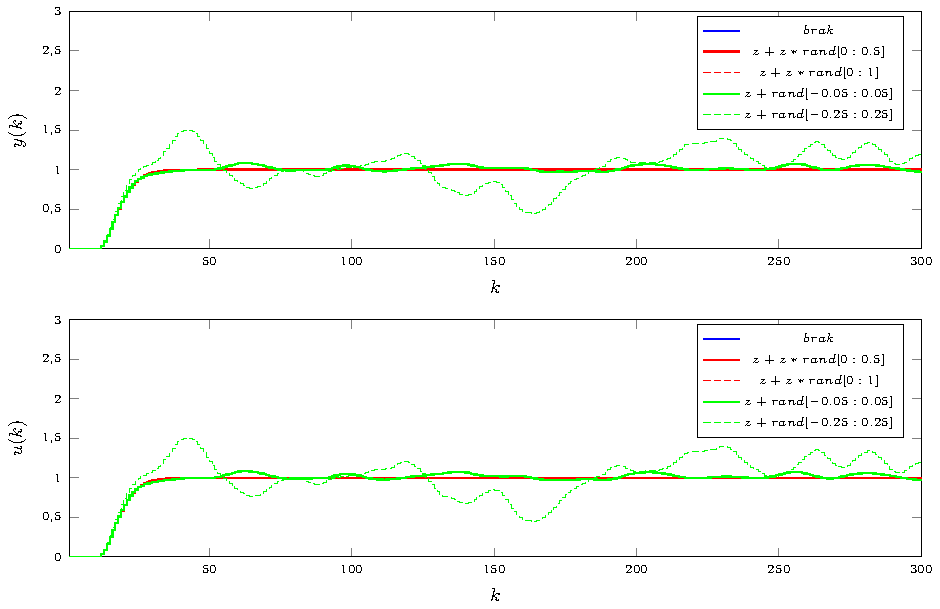
\includegraphics[scale=1.4]{../wykresy_pdf/zad7_dmc_blad1.pdf}
\caption {Symulacja algorytmu DMC dla przy szumie pomiarowym i zerowym zak��ceniu}
\label{dmc_szum_0}
\end{figure}

\begin{figure}[b]
\centering
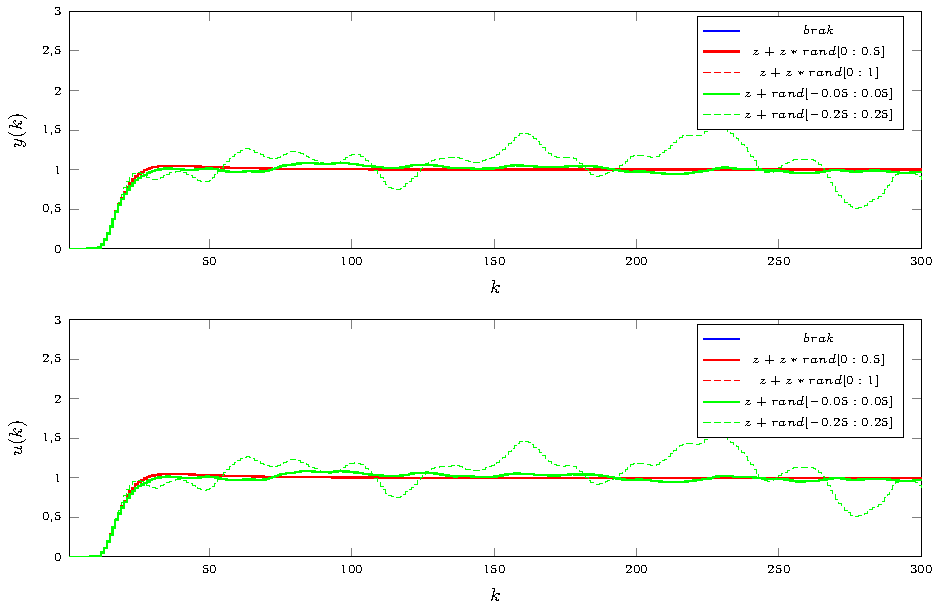
\includegraphics[scale=1.4]{../wykresy_pdf/zad7_dmc_blad2.pdf}
\caption {Symulacja algorytmu DMC dla przy szumie pomiarowym i sta�ym niezerowym zak��ceniu}
\label{dmc_szum_stale}
\end{figure}

\begin{figure}[b]
\centering
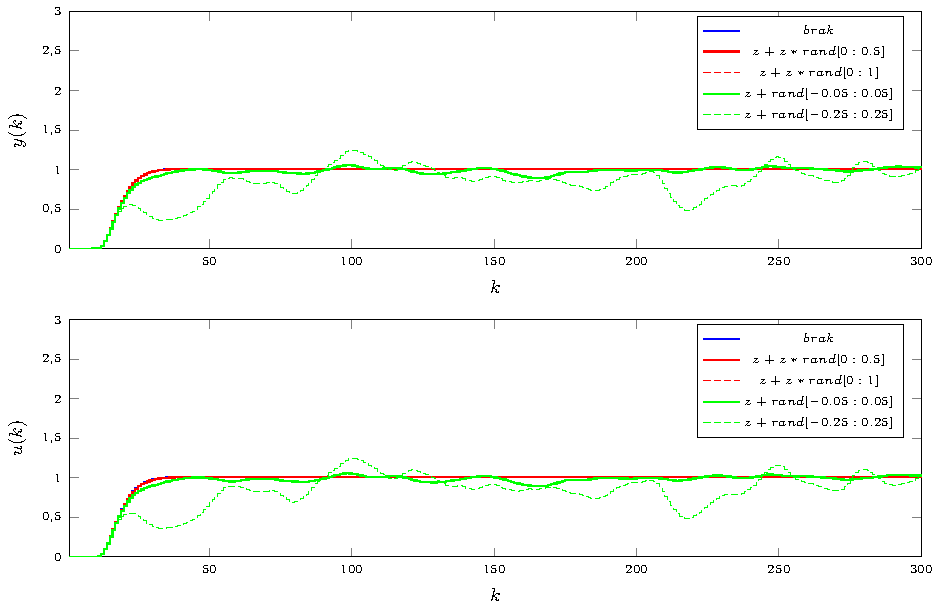
\includegraphics[scale=1.4]{../wykresy_pdf/zad7_dmc_blad3.pdf}
\caption {Symulacja algorytmu DMC dla przy szumie pomiarowym i zak��ceniu rosn�cym liniowo}
\label{dmc_szum_lin}
\end{figure}
\end{document}


